%%%%%%%%%%%%%%%%%%%%%%%%%%%%%%%%%%%%%%%%%
% Stylish Article
% LaTeX Template
% Version 2.2 (2020-10-22)
%
% This template has been downloaded from:
% http://www.LaTeXTemplates.com
%
% Original author:
% Mathias Legrand (legrand.mathias@gmail.com) 
% With extensive modifications by:
% Vel (vel@latextemplates.com)
%
% License:
% CC BY-NC-SA 3.0 (http://creativecommons.org/licenses/by-nc-sa/3.0/)
%
%%%%%%%%%%%%%%%%%%%%%%%%%%%%%%%%%%%%%%%%%

%----------------------------------------------------------------------------------------
%	PACKAGES AND OTHER DOCUMENT CONFIGURATIONS
%----------------------------------------------------------------------------------------

\documentclass[fleqn,11pt]{SelfArx} % Document font size and equations flushed left

\usepackage[spanish]{babel} % Specify a different language here - english by default

\usepackage{lipsum} % Required to insert dummy text. To be removed otherwise

%----------------------------------------------------------------------------------------
%	COLUMNS
%----------------------------------------------------------------------------------------

\setlength{\columnsep}{0.55cm} % Distance between the two columns of text
\setlength{\fboxrule}{0.75pt} % Width of the border around the abstract

%----------------------------------------------------------------------------------------
%	COLORS
%----------------------------------------------------------------------------------------

\definecolor{color1}{RGB}{0,0,90} % Color of the article title and sections
\definecolor{color2}{RGB}{0,20,20} % Color of the boxes behind the abstract and headings

%----------------------------------------------------------------------------------------
%	HYPERLINKS
%----------------------------------------------------------------------------------------

\usepackage{hyperref} % Required for hyperlinks

\hypersetup{
	hidelinks,
	colorlinks,
	breaklinks=true,
	urlcolor=color2,
	citecolor=color1,
	linkcolor=color1,
	bookmarksopen=false,
	pdftitle={Title},
	pdfauthor={Author},
}

%----------------------------------------------------------------------------------------
%	ARTICLE INFORMATION
%----------------------------------------------------------------------------------------

\JournalInfo{Laboratorio de Electricidad y Magnetismo} % Journal information
\Archive{\textsuperscript\textcopyleft 2022 Ceballiguel} % Additional notes (e.g. copyright, DOI, review/research article)

\PaperTitle{Ciclo de Histéresis} % Article title

\Authors{F. J. Ceballos\textsuperscript{1$\dagger$}, M. de Miguel\textsuperscript{1}*} % Authors
\affiliation{\textsuperscript{1}\textit{Facultad de CC. Físicas, Universidad Complutense de Madrid, Madrid, España}} % Author affiliation
\affiliation{\textsuperscript{$\dagger$}franceba@ucm.es,  *mdemig02@ucm.es} % Corresponding author

\Keywords{Sus --- Amongus --- Miguel} % Keywords - if you don't want any simply remove all the text between the curly brackets
\newcommand{\keywordname}{Keywords} % Defines the keywords heading name

%----------------------------------------------------------------------------------------
%	ABSTRACT
%----------------------------------------------------------------------------------------

\Abstract{}

%----------------------------------------------------------------------------------------

\begin{document}

\maketitle % Output the title and abstract box

\tableofcontents % Output the contents section

\thispagestyle{empty} % Removes page numbering from the first page

%----------------------------------------------------------------------------------------
%	ARTICLE CONTENTS
%----------------------------------------------------------------------------------------

\section*{Introducción} % The \section*{} command stops section numbering

\addcontentsline{toc}{section}{Introduction} % Adds this section to the table of contents



%------------------------------------------------

\section{Método experimental}

\begin{figure*}[ht]\centering % Using \begin{figure*} makes the figure take up the entire width of the page
	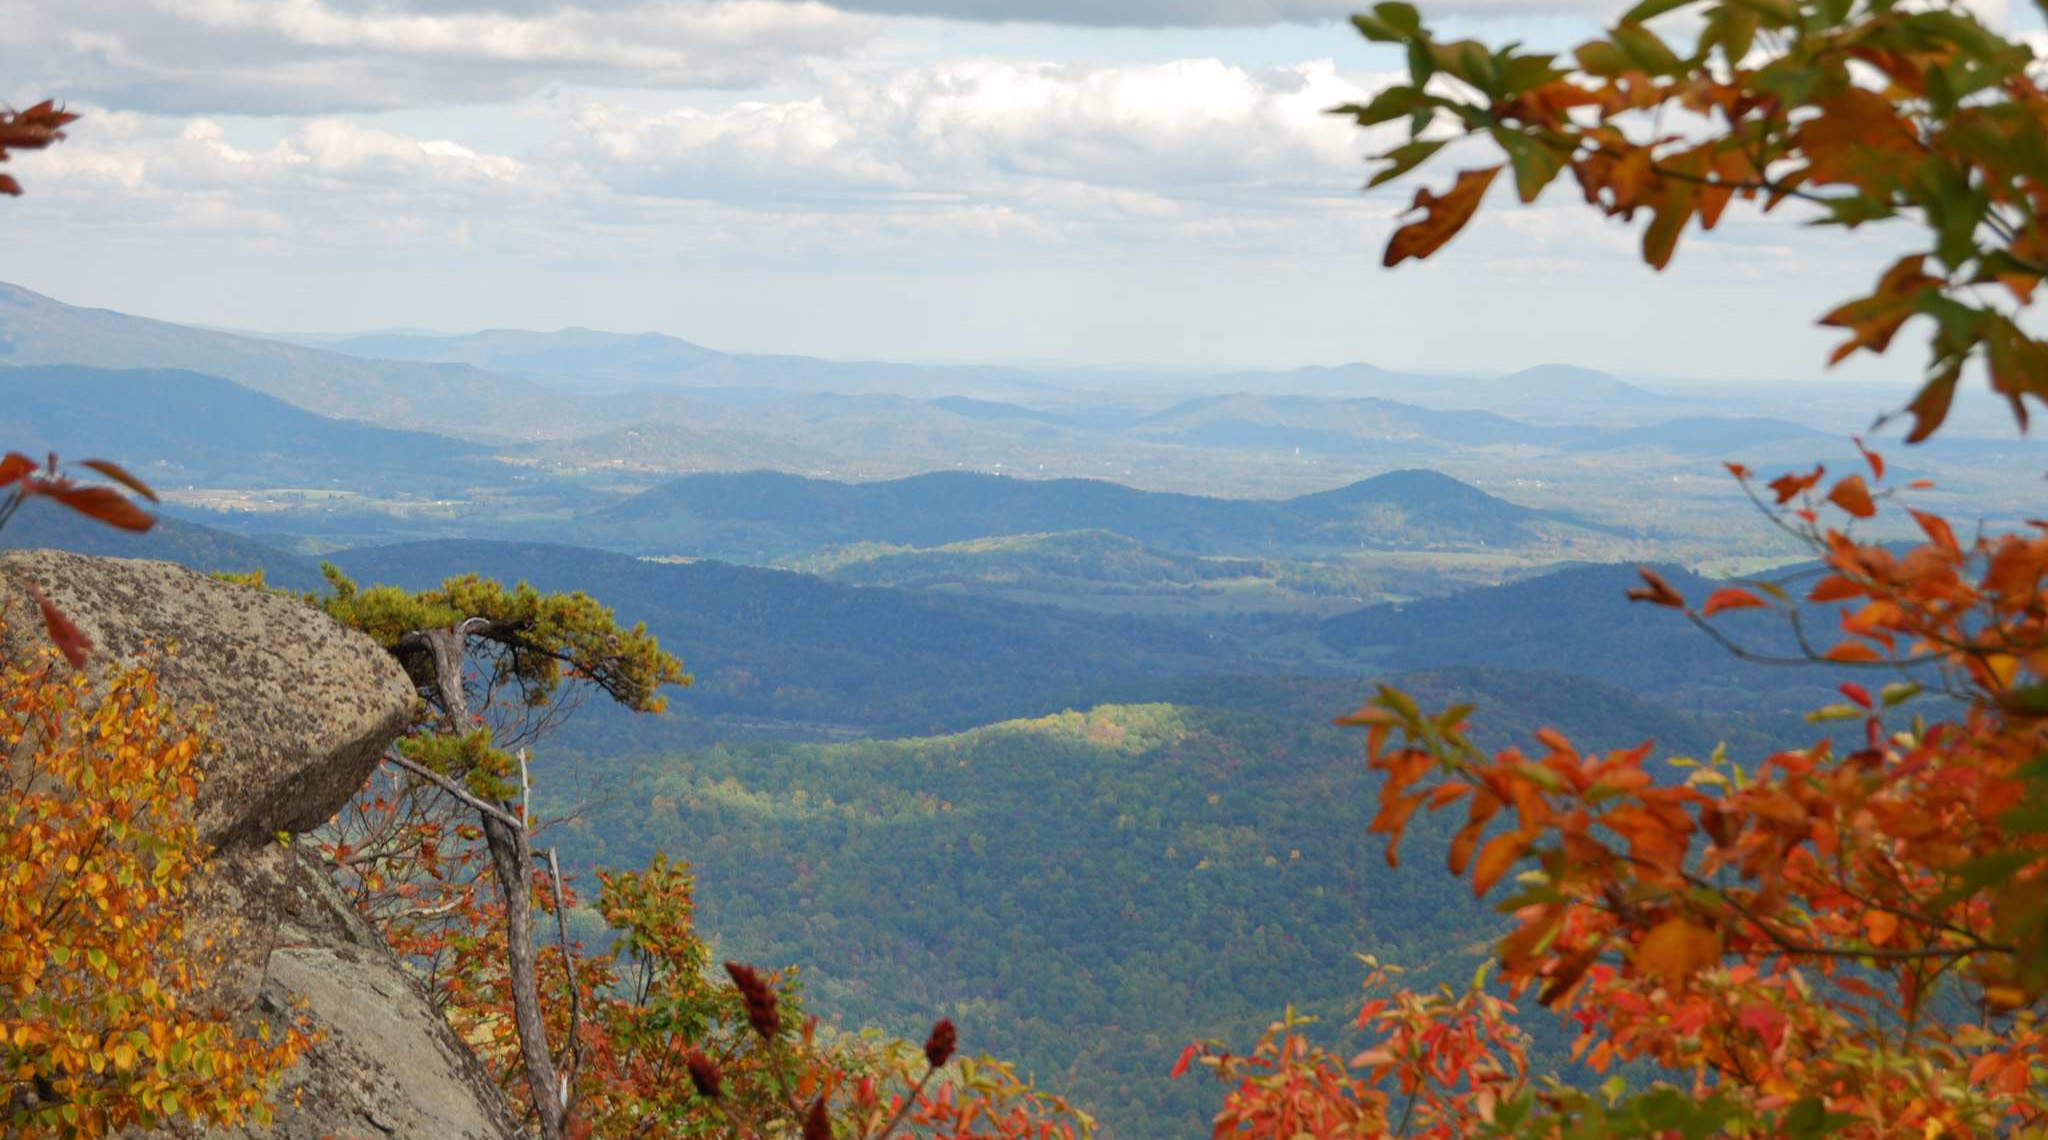
\includegraphics[width=\linewidth]{view}
	\caption{Wide Picture}
	\label{fig:view}
\end{figure*}

\lipsum[4] % Dummy text

\begin{equation}
	\cos^3 \theta =\frac{1}{4}\cos\theta+\frac{3}{4}\cos 3\theta
	\label{eq:refname2}
\end{equation}

\lipsum[5] % Dummy text

\begin{enumerate}[noitemsep] % [noitemsep] removes whitespace between the items for a compact look
	\item First item in a list
	\item Second item in a list
	\item Third item in a list
\end{enumerate}

\subsection{Subsection}

\lipsum[6] % Dummy text

\paragraph{Paragraph} \lipsum[7] % Dummy text
\paragraph{Paragraph} \lipsum[8] % Dummy text

\subsection{Subsection}

\lipsum[9] % Dummy text

\begin{figure}[ht]\centering
	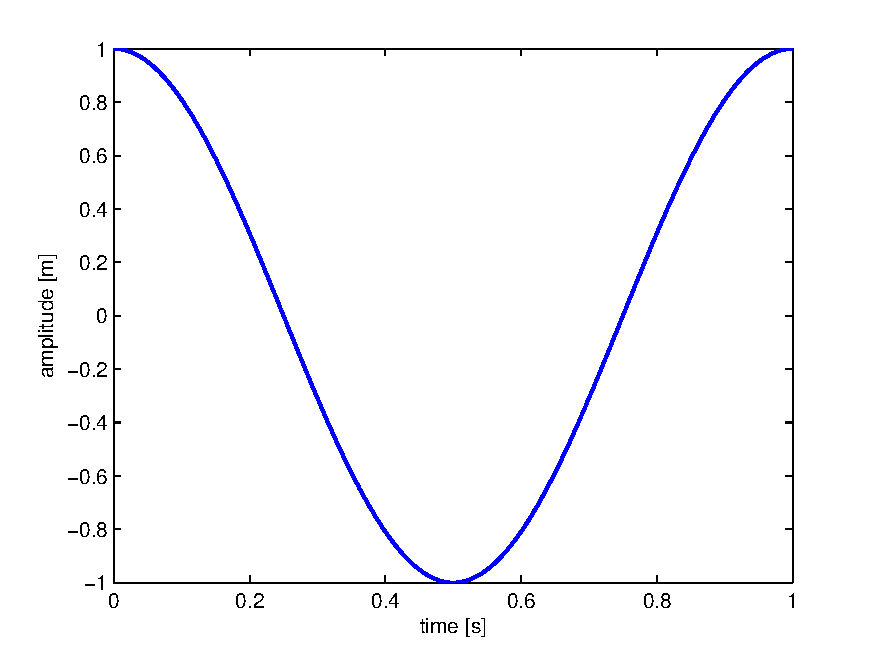
\includegraphics[width=\linewidth]{results}
	\caption{In-text Picture}
	\label{fig:results}
\end{figure}

Reference to Figure \ref{fig:results}.

%------------------------------------------------

\section{Results and Discussion}

\lipsum[10] % Dummy text

\subsection{Subsection}

\lipsum[11] % Dummy text

\begin{table}[hbt]
	\caption{Table of Grades}
	\centering
	\begin{tabular}{llr}
		\toprule
		\multicolumn{2}{c}{Name} \\
		\cmidrule(r){1-2}
		First name & Last Name & Grade \\
		\midrule
		John & Doe & $7.5$ \\
		Richard & Miles & $2$ \\
		\bottomrule
	\end{tabular}
	\label{tab:label}
\end{table}

\subsubsection{Subsubsection}

\lipsum[12] % Dummy text

\begin{description}
	\item[Word] Definition
	\item[Concept] Explanation
	\item[Idea] Text
\end{description}

\subsubsection{Subsubsection}

\lipsum[13] % Dummy text

\begin{itemize}[noitemsep] % [noitemsep] removes whitespace between the items for a compact look
	\item First item in a list
	\item Second item in a list
	\item Third item in a list
\end{itemize}

\subsubsection{Subsubsection}

\lipsum[14] % Dummy text

\subsection{Subsection}

\lipsum[15-23] % Dummy text

%------------------------------------------------

\phantomsection
\section*{Acknowledgments} % The \section*{} command stops section numbering

\addcontentsline{toc}{section}{Acknowledgments} % Adds this section to the table of contents

So long and thanks for all the fish \cite{Figueredo:2009dg, Smith:2012qr}.

%----------------------------------------------------------------------------------------
%	REFERENCE LIST
%----------------------------------------------------------------------------------------

\phantomsection
\bibliographystyle{unsrt}
\bibliography{sample.bib}

%----------------------------------------------------------------------------------------

\end{document}